\documentclass[11pt]{article}
\usepackage[margin=0.9in]{geometry}
\usepackage{amsmath,amssymb}
\usepackage{booktabs}
\usepackage{graphicx}
\usepackage{fancyhdr}
\usepackage[hidelinks]{hyperref}

\graphicspath{{Figures/}}
\pagestyle{fancy}
\fancyhf{}
\lhead{STAT 546 \textbar{} HW4 implementation report \textbar{} Anurag Ramesh}
\rhead{16 October 2026}
\cfoot{\thepage}
\renewcommand{\headrulewidth}{0.4pt}
\setlength{\parindent}{0pt}
\setlength{\parskip}{6pt}

\begin{document}

All code is in \texttt{Scripts/}, one script per question. Each script uses the general samplers in the
project root (\texttt{SAMC.py}, built on \texttt{Metropolis\_Hastings.py}) and saves its figure in
\texttt{Figures/} and its numbers in \texttt{Results/}.

\section*{SAMC, as used in all four questions}

All four questions use stochastic approximation Monte Carlo (SAMC; Liang, Liu and Carroll, 2007). Each
question samples from a target $\psi(x) = \exp(-U(x)/\tau)$, where $U$ is an energy and $\tau$ a
temperature. The sample space is split into subregions $E_1, \ldots, E_m$ by a chosen quantity (tour length,
energy, or $|t|$), and $J(x)$ denotes the subregion of $x$. Each subregion has a log weight $\theta_i$, starting
at 0. SAMC runs MH on the working density
\[
p_\theta(x) \propto \exp\left(-U(x)/\tau - \theta_{J(x)}\right).
\]
All proposals used here are symmetric, so a proposed state $y$ is accepted with probability
\[
\alpha = \min\left\{1, \exp\left[-\frac{U(y) - U(x)}{\tau} + \theta_{J(x)} - \theta_{J(y)}\right]\right\}.
\]
After each step, with $x_t$ the current state, every weight is updated as
\[
\theta_i \leftarrow \theta_i + \gamma_t \left( \mathbf{1}\{i = J(x_t)\} - \pi_i \right), \qquad
\gamma_t = \frac{t_0}{\max(t_0, t)},
\]
where $\pi_i = 1/m$ is the desired share of time in each subregion. The weight of the subregion the chain is in
goes up, which makes that subregion less attractive. A chain stuck in one mode or local minimum is therefore
pushed out of it, and in the long run it spends about a $1/m$ share of time in every subregion it can reach.

The results are used in two ways.

\textbf{Optimization (Q1, Q2).} The lowest-energy state visited is saved.

\textbf{Estimation (Q3, Q4).} The samples follow the working density, not $\psi$. Each stored sample $x_t$ gets
the importance weight $w_t = \exp(\theta_{J(x_t)})$, using the weights at that iteration, and an expectation
under $\psi$ is estimated by the weighted average
\[
\widehat{E}[h(x)] = \frac{\sum_t w_t\, h(x_t)}{\sum_t w_t}.
\]

\newpage
\section*{Q1. SAMC for 100-city tours}

I interpreted the requested average as an average over independently generated city sets. I generated 20 sets,
each containing 100 cities sampled uniformly from $[0, 100] \times [0, 100]$ miles, and ran SAMC once on each
set from a random tour.

A tour is an ordering of all 100 cities. Its energy is its length $L$: the sum of Euclidean distances between
consecutive cities, including the return from the last city to the first. Each proposal reverses one segment
of the tour (a 2-opt move), so it keeps every city exactly once.

I split the tours by length into $m = 61$ subregions, using the levels $700, 705, \ldots, 995$ miles:
$E_1 = \{L \le 700\}$, 5-mile subregions in between, and $E_{61} = \{L > 995\}$. The shortest tour visited is
saved.

\begin{center}
\begin{tabular}{p{0.45\textwidth}p{0.45\textwidth}}
\toprule
\textbf{Setting / result} & \textbf{Value} \\
\midrule
City sets / seed & 20 / 546 \\
Iterations per set & 1,000,000 \\
Temperature $\tau$ / gain constant $t_0$ & 2 / 5,000 \\
Subregions & 61, with 5-mile levels from 700 to 995 miles \\
\textbf{Average shortest tour across 20 sets} & \textbf{787.7 miles} \\
\bottomrule
\end{tabular}
\end{center}

These are the shortest tours found within the stated budget. Their true optimality is not certified, so the
average may be slightly above the average of the exact shortest tours.

\begin{center}
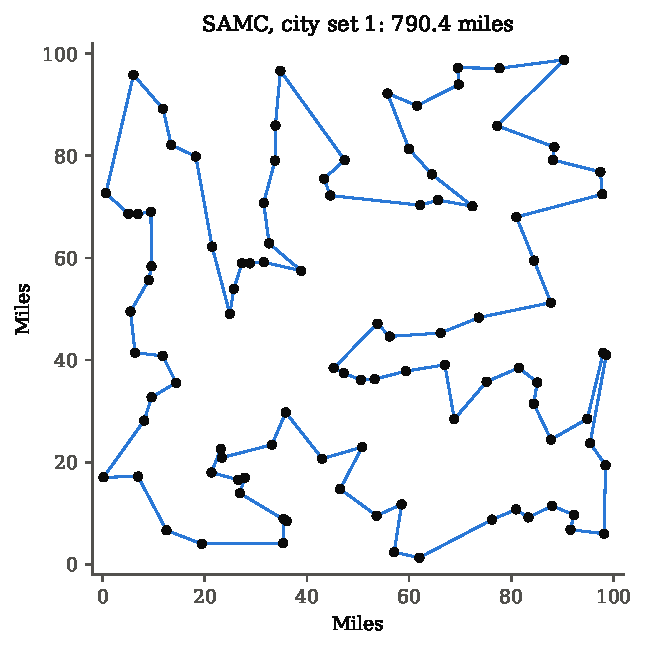
\includegraphics[width=0.5\textwidth]{q1_samc_tsp.pdf}
\end{center}

\newpage
\section*{Q2. Simulated stochastic approximation annealing for 100-city tours}

I used the same 20 city sets, the same 2-opt moves and the same 61 subregions as in Q1. Simulated stochastic
approximation annealing (SAA; Liang, Cheng and Lin, 2014) is SAMC whose temperature is lowered during the run. At iteration $t$ the working
density is
\[
p_{\theta, t}(x) \propto \exp\left(-L(x)/\tau_t - \theta_{J(x)}\right),
\qquad
\tau_t = T_{\text{high}} \sqrt{\frac{t_c}{\max(t_c, t)}},
\]
so the temperature falls with the square root of the iteration number. The acceptance probability and the
weight update are the SAMC ones, with $\tau_t$ in place of $\tau$. The weights still push the chain out of
subregions it stays in, while the falling temperature concentrates it on shorter tours. The shortest tour
visited is saved.

\begin{center}
\begin{tabular}{p{0.45\textwidth}p{0.45\textwidth}}
\toprule
\textbf{Setting / result} & \textbf{Value} \\
\midrule
City sets / seed & 20 / 546 (as in Q1) \\
Iterations per set & 1,000,000 \\
Cooling & $T_{\text{high}} = 10$, $t_c = 1{,}000$; $\tau$ falls from 10 to 0.32 \\
Gain constant $t_0$ / subregions & 5,000 / 61 (as in Q1) \\
\textbf{Average shortest tour across 20 sets} & \textbf{787.4 miles} \\
\bottomrule
\end{tabular}
\end{center}

As in Q1, the shortest tours found are not certified optimal.

\begin{center}
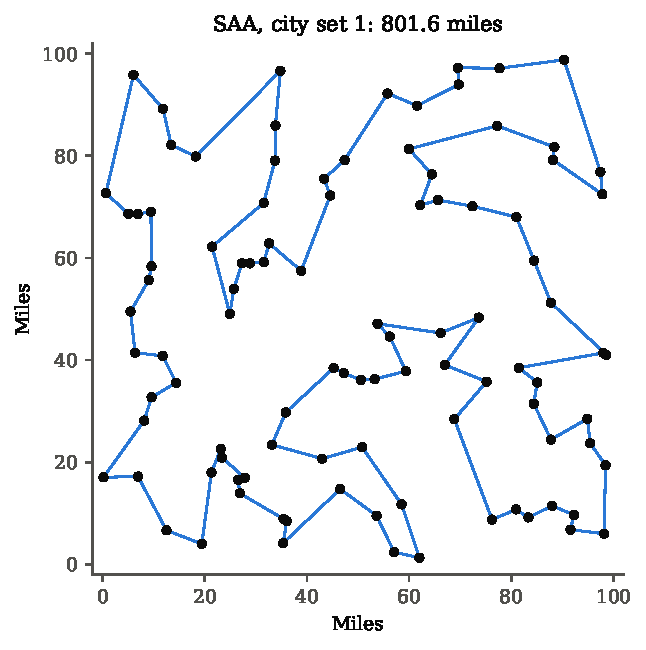
\includegraphics[width=0.5\textwidth]{q2_saa_tsp.pdf}
\end{center}

\newpage
\section*{Q3. SAMC for the mean and covariance of the normal mixture}

The target is $f(x) = \frac{1}{3}N(\mu_1, \Sigma_1) + \frac{1}{3}N(\mu_2, \Sigma_2) + \frac{1}{3}N(\mu_3, \Sigma_3)$
exactly as given. Its three modes are far apart, so a plain random-walk MH chain would rarely move between
them.

I used the energy $U(x) = -\log f(x)$ with $\tau = 1$, so $\psi = f$, and split the plane by energy into
$m = 14$ subregions with levels $2.5, 3.5, \ldots, 14.5$: $E_1 = \{U \le 2.5\}$, unit-width subregions in
between, and $E_{14} = \{U > 14.5\}$. Each proposal is a normal random move. Because the chain spends about a
$1/14$ share of time in every subregion, including the high-energy ones between the modes, it crosses between
the modes regularly.

The mean and covariance are the weighted averages from the SAMC section:
\[
\hat{\mu} = \frac{\sum_t w_t x_t}{\sum_t w_t}, \qquad
\hat{\Sigma} = \frac{\sum_t w_t (x_t - \hat{\mu})(x_t - \hat{\mu})^T}{\sum_t w_t}.
\]
The exact values are $\mu = \frac{1}{3}(\mu_1 + \mu_2 + \mu_3)$ and
$\Sigma = \frac{1}{3}\sum_k (\Sigma_k + \mu_k \mu_k^T) - \mu \mu^T$, which give a direct check.

\begin{center}
\begin{tabular}{p{0.45\textwidth}p{0.45\textwidth}}
\toprule
\textbf{Setting} & \textbf{Value} \\
\midrule
Iterations / discarded / seed & 4,000,000 / 400,000 / 546 \\
Stored samples & Every 10th state after burn-in \\
Normal proposal standard deviation / $t_0$ & 1.5 / 1,000 \\
\bottomrule
\end{tabular}
\end{center}

\begin{center}
\begin{tabular}{lcc}
\toprule
\textbf{Quantity} & \textbf{SAMC estimate} & \textbf{Exact} \\
\midrule
Mean $\mu$ & $(-0.649, -0.640)$ & $(-0.667, -0.667)$ \\[2pt]
Covariance $\Sigma$ & $\begin{pmatrix} 33.819 & 32.857 \\ 32.857 & 33.898 \end{pmatrix}$
  & $\begin{pmatrix} 33.889 & 32.889 \\ 32.889 & 33.889 \end{pmatrix}$ \\
\bottomrule
\end{tabular}
\end{center}

\begin{center}
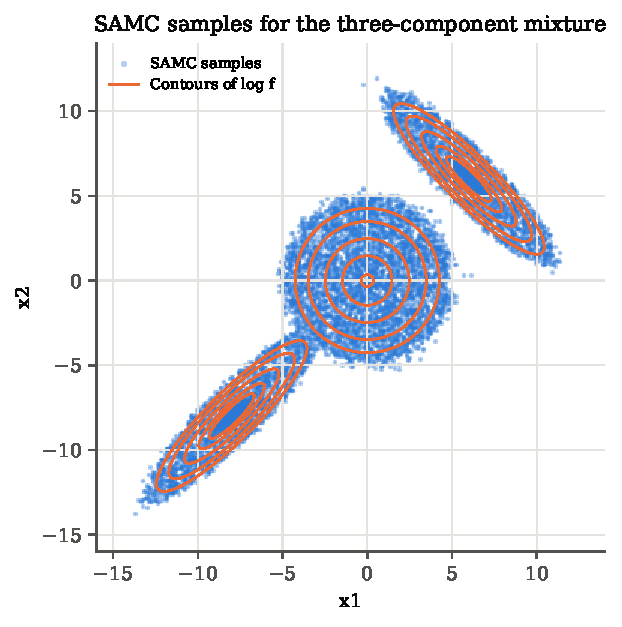
\includegraphics[width=0.48\textwidth]{q3_samc_mixture.pdf}
\end{center}

\newpage
\section*{Q4. SAMC for p-values of the two-sample t-test}

\subsection*{Data and p-value}

The assignment does not supply data. I simulated $n_1 = 12$ observations from $N(0, 1)$ and $n_2 = 12$ from
$N(2, 1)$, with seed 546; the values are saved with the results. The test statistic is the pooled two-sample
$t$-statistic, and its observed value is $|t_{\text{obs}}| = 4.696$.

I evaluated the permutation p-value: the fraction of all ways of splitting the 24 values into groups of 12 and
12 whose $|t|$ is at least $|t_{\text{obs}}|$. Under the null hypothesis every split is equally likely. There are
$\binom{24}{12} = 2{,}704{,}156$ splits, few enough to list them all, which gives the exact p-value as a check.

\subsection*{SAMC}

Using SAMC to evaluate small p-values of resampling-based tests was proposed by Yu et al.\ (2011). The state is
a split of the data. Each proposal swaps one randomly chosen member of group 1 with one randomly
chosen member of group 2. The target is uniform on the splits, so the energy is 0 and the acceptance
probability is $\min\{1, \exp(\theta_{J(x)} - \theta_{J(y)})\}$.

I divided the splits by $|t|$ into $m = 24$ subregions: 23 equal-width subregions covering
$[0, |t_{\text{obs}}|)$, and the tail $E_{24} = \{|t| \ge |t_{\text{obs}}|\}$. Because the chain spends about a
$1/24$ share of time in every subregion, it visits the tail often even though the tail holds very few splits.
The p-value is the weighted average from the SAMC section with $h(x) = \mathbf{1}\{x \in E_{24}\}$:
\[
\hat{p} = \frac{\sum_t w_t\, \mathbf{1}\{x_t \in E_{24}\}}{\sum_t w_t}.
\]

\begin{center}
\begin{tabular}{p{0.45\textwidth}p{0.45\textwidth}}
\toprule
\textbf{Setting / result} & \textbf{Value} \\
\midrule
Iterations / discarded / seed & 1,000,000 / 100,000 / 546 \\
Stored samples / gain constant $t_0$ & Every 10th state after burn-in / 300 \\
\textbf{SAMC p-value} & \textbf{$7.32 \times 10^{-5}$} \\
\textbf{Exact permutation p-value} & \textbf{$7.69 \times 10^{-5}$} \\
\bottomrule
\end{tabular}
\end{center}

\begin{center}
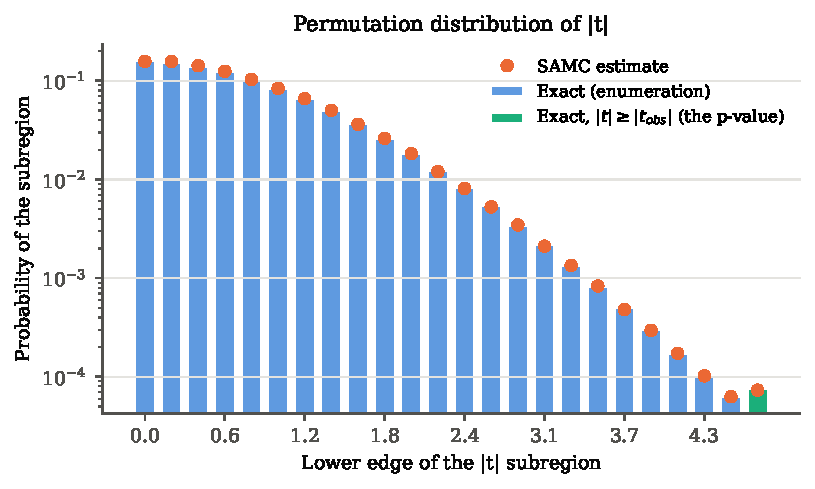
\includegraphics[width=0.62\textwidth]{q4_samc_pvalue.pdf}
\end{center}

\newpage
\section*{References}

STAT 546, Fall 2026. Homework 4, Questions 1--4. The problems and requested algorithms are taken from the
assignment.

F. Liang, C. Liu and R. J. Carroll (2007). Stochastic approximation in Monte Carlo computation. \emph{Journal of
the American Statistical Association}, 102, 305--320. DOI:
\href{https://doi.org/10.1198/016214506000001202}{10.1198/016214506000001202}.

F. Liang, Y. Cheng and G. Lin (2014). Simulated stochastic approximation annealing for global optimization with
a square-root cooling schedule. \emph{Journal of the American Statistical Association}, 109(506), 847--863.
DOI: \href{https://doi.org/10.1080/01621459.2013.872993}{10.1080/01621459.2013.872993}.

K. Yu, F. Liang, J. Ciampa and N. Chatterjee (2011). Efficient p-value evaluation for resampling-based tests.
\emph{Biostatistics}, 12(3), 582--593. DOI:
\href{https://doi.org/10.1093/biostatistics/kxq078}{10.1093/biostatistics/kxq078}.

\end{document}
